\chapter{从局部误差到当前状态：ESKF直观}

\label{chap:md-08}

前面几章分别建立了状态空间、局部坐标、李群扰动和概率的语言。现在把它们放到一台带IMU的机器人身上：IMU不断给出读数，机器人先据此预测自己走到了哪里；外部传感器随后提供新观测，估计再向能够解释观测的状态移动。这一过程持续回答两个问题：当前先按哪个状态计算？这个状态附近还允许怎样的偏离？

本章只追踪当前状态的估计。先给出三维姿态、位置、速度和偏置，再沿“名义状态预测—误差与协方差传播—观测修正—注入与重置”走完一次ESKF循环。矩阵暂时被看作有明确输入、输出的局部映射；下一章再从真实与名义运动出发逐项推导。区间IMU的预积分从第\ref{chap:md-10}章开始讨论。

\section{前面的数学怎样成为一个状态估计}

\subsection{状态是一个点，不确定性分配给区域}

沿用前几章的观点，真实状态是状态空间$M$中的一个点$x$。我们不知道这个点在哪里，所以还需要在$M$的可测区域上给出概率。比如"位置在这一小片区域内，同时姿态在某个范围内"是一个事件；它的概率表达当前信息对这一片可能状态的支持程度。

一个估计值不能独自表达这件事。两次估计都报出同一个位置，其中一次可能很有把握，另一次可能允许很大的偏离。因此我们同时保存一个参考状态$\hat x$和它附近的不确定性。参考状态称为\textbf{名义状态}，可以理解为"当前先按它来计算的那个合法状态"。

本章使用的惯性导航状态为

\begin{equation*}
x=(R,p,v,b_g,b_a)\in M=\mathcal X:=\mathop{\mathrm{SO}}(3)\times\mathbb R^{12}.
\end{equation*}

$R$是姿态，$p$是位置，$v$是速度，$b_g,b_a$分别是陀螺仪和加速度计偏置。每个向量有三个分量；姿态也有三个局部自由度，所以状态共有十五个局部自由度。地图暂时不放进这个状态，看到的路标先当作已知。

\subsection{用局部误差描述参考点附近的可能状态}

我们需要一种方式，从$\hat x$出发描述附近的$x$。位置、速度、偏置可以相加，姿态使用第\ref{chap:md-06}章的小旋转：

\begin{equation}\label{eq-intuition-oplus}
\begin{aligned}
 R&=\hat R\mathop{\mathrm{Exp}}(\delta\theta^\wedge),&p&=\hat p+\delta p,\\
 v&=\hat v+\delta v,&b_g&=\hat b_g+\delta b_g,\\
 &&b_a&=\hat b_a+\delta b_a.
\end{aligned}
\end{equation}

把这五种局部偏离依次排成列向量，记为

\begin{equation*}
\delta x=(\delta\theta^\top,\delta p^\top,\delta v^\top,
                \delta b_g^\top,\delta b_a^\top)^\top\in\mathbb R^{15}.
\end{equation*}

上式整体简记为$x=\hat x\oplus\delta x$。$\oplus$不是把所有状态都当作普通向量相加，而是约定使用式\eqref{eq-intuition-oplus}的局部更新规则。

这里$\delta\theta$是三维小旋转坐标，$\delta\theta^\wedge$是对应的叉积矩阵，满足$\delta\theta^\wedge u=\delta\theta\times u$；$\hat R\delta\theta^\wedge$才是$T_{\hat R}\mathop{\mathrm{SO}}(3)$中的切向量。$\mathop{\mathrm{Exp}}$将小旋转变成群元素，右乘后仍是合法旋转。这就把"切空间里算增量、流形上更新状态"的数学语言落实为一次实际操作。

帽号$\hat R$表示估计，右上角$\wedge$表示把向量变成叉积矩阵。若反过来比较真实姿态和名义姿态，在局部有

\begin{equation*}
\delta\theta=\mathop{\mathrm{Log}}(\hat R^\top R)^\vee.
\end{equation*}

先求相对旋转，再取对数与$\vee$得到向量；这里固定使用右侧误差，后面不再更换约定。

\subsection{把概率模型放在这组误差坐标上}

采用局部高斯近似：

\begin{equation}\label{eq-intuition-local-gaussian}
\boxed{x=\hat x\oplus\delta x,\qquad\delta x\sim\mathcal N(0,P).}
\end{equation}

$P$是十五维误差的协方差。它既记录每一种偏离有多大，也记录哪些偏离倾向于一起出现。例如姿态方向略有偏差，会影响速度和位置的预测，这种联系也要保存在$P$中。

按第\ref{chap:md-07}章的语言，局部误差的概率分布通过$\delta x\mapsto\hat x\oplus\delta x$送到状态空间。想知道状态落在某区域$A$的概率，就看哪些误差向量会被送进$A$。因此高斯写在局部向量上，概率最终描述的仍是可能状态的区域。

误差均值为零，表示当前用$\hat x$作为分布中心；某一次真实误差$\delta x$通常仍未知，也不一定为零。后面由观测算出的$\widehat{\delta x}$只是对误差的估计，不能与真实误差混为一谈。这个近似适用于不确定性集中在参考状态附近的情形。

还要记住：协方差依赖误差坐标。若同一偏离改写为$e'=Ce$，则

\begin{equation*}
\operatorname{Cov}(e')=C\operatorname{Cov}(e)C^\top.
\end{equation*}

这是第\ref{chap:md-07}章的二阶矩经过线性映射后的结果。稍后的预测和重置都会使用它：前者让偏离随运动向前变化，后者改变描述偏离的参考点。

\section{IMU怎样推动名义状态}

\subsection{先固定向量在哪个坐标系中}

$R=R_{WB}$把机体系$B$中的向量送到世界系$W$，例如$a_W=Ra_B$；$R^\top$做反向变换。位置$p$、速度$v$和重力$g_W$都用世界系表达，IMU读数和偏置沿传感器自身的三个轴表达。本章假设IMU与机体系重合，重力是已知常向量。

机器人转动时，传感器的轴也跟着转。沿传感器轴测出的向量必须先乘$R$，才能与世界系的速度变化和重力放在同一个等式中。这是姿态为什么会参与平移预测的直接原因。

\subsection{读数、偏置与真实输入}

记陀螺读数为$\omega_m$，加速度计读数为$a_m$，测量模型为

\begin{equation*}
\omega_m=\omega+b_g+n_g,\qquad a_m=a+b_a+n_a.
\end{equation*}

$\omega$是机体系角速度，$a$是机体系比力，$n_g,n_a$是零均值测量噪声。偏置是缓慢变化的系统偏移，需要作为状态估计；噪声则表示每次读数中未知的随机部分。

加速度计的比力满足$a=R^\top(\dot v-g_W)$。因此真实运动遵循

\begin{equation*}
\dot R=R\omega^\wedge,\qquad\dot p=v,\qquad\dot v=g_W+Ra.
\end{equation*}

速度方程可以逐步读成：去掉读数中的偏置与噪声，得到比力；用姿态转到世界系；加上重力，得到速度变化率。静止时$\dot v=0$，所以理想读数$a=-R^\top g_W$，通常不为零。

\subsection{当前先按名义状态往前算}

真实偏置和噪声未知。实际计算先扣除当前偏置估计，记

\begin{equation*}
\hat\omega_k=\omega_{m,k}-\hat b_{g,k},\qquad
 \hat a_k=a_{m,k}-\hat b_{a,k}.
\end{equation*}

帽号表示这一步采用的输入。对于很短的一步$h=\Delta t_k=t_{k+1}-t_k$，用起点姿态近似步内比力的世界方向，得到

\begin{equation}\label{eq-eskf-nominal-step}
\begin{aligned}
 \hat R_{k+1}^-&=\hat R_k^+\mathop{\mathrm{Exp}}((\hat\omega_kh)^\wedge),\\
 \hat p_{k+1}^-&=\hat p_k^++\hat v_k^+h
                 +\tfrac12(g_W+\hat R_k^+\hat a_k)h^2,\\
 \hat v_{k+1}^-&=\hat v_k^++(g_W+\hat R_k^+\hat a_k)h,\\
 \hat b_{g,k+1}^-&=\hat b_{g,k}^+,
 \qquad\hat b_{a,k+1}^-=\hat b_{a,k}^+.
\end{aligned}
\end{equation}

上标$-$表示外部观测到来前的预测，$+$表示完成观测修正后的估计，不是数值的正负号。没有外部观测时，就直接把预测接到下一步。

旋转由角速度乘时间得到小旋转，再通过群乘法复合。位置和速度则沿熟悉的运动学关系前进，位置式使用旧速度，因为本步加速度的贡献已经由$\tfrac12h^2$项另行计算。偏置名义值暂时不变，表示没有新信息表明它会向某个方向漂移；偏置的不确定性仍会增长。

\begin{bookexample}{用静止状态检查这一步}

世界系$z$轴向上，取$\hat R=I$、$g_W=(0,0,-g)^\top$。去偏置的静止读数为$\hat a=(0,0,g)^\top$，于是$g_W+\hat R\hat a=0$。若初速为零，位置和速度保持不变。这个检查同时说明了比力、坐标变换和重力加回各自的作用。

\end{bookexample}

这组递推是选定的数值近似：步内转动明显时，旋转后的比力会变化。下一章以同一组递推推导对应的误差和噪声矩阵，使名义传播与协方差传播相互匹配。

\section{预测时，误差和不确定性怎样一起向前走}

\subsection{想象两条彼此接近的轨迹}

一条轨迹从名义状态出发，使用当前采用的输入；另一条是真实轨迹，起点有小偏离，输入还受到偏置误差与噪声影响。下一时刻的误差，就是这两条轨迹走完同一小段时间后，在新参考点附近的差。

先不拆开所有分量，只保留一阶关系：

\begin{equation}\label{eq-intuition-error-step}
\boxed{\delta x_{k+1}\simeq\Phi_k\delta x_k+w_k.}
\end{equation}

$\Phi_k$是十五维旧误差到新误差的线性映射：它回答"起点稍微偏一点，终点会怎样偏"。这是第\ref{chap:md-05}章的微分在局部坐标中的矩阵表示。$w_k$收集这一时间段新进入的随机扰动，记其协方差为$Q_{d,k}$；下标$d$提醒我们它已经是\textbf{整步噪声增量}的协方差。

例如，旧速度稍大，下一步位置也会偏大；姿态略微倾斜，本来接近竖直的比力会出现水平投影，之后影响速度与位置。这些关系由$\Phi_k$一起记录。现在只需理解它传递了哪些影响，下一章再从两条轨迹的方程中逐项算出它。

\subsection{旧的不确定性被传播，新的噪声被加入}

当旧误差和本步噪声独立、零均值时，把式\eqref{eq-intuition-error-step}代入协方差定义即可得到

\begin{equation}\label{eq-intuition-p-predict}
\boxed{P_{k+1}^-=\Phi_kP_k^+\Phi_k^\top+Q_{d,k}.}
\end{equation}

第一项让已有误差分布随运动改变，第二项加入本时间段的新不确定性。前者接上微分的局部传播，二者相加则来自第\ref{chap:md-07}章关于独立随机量二阶矩的计算。

因此一次IMU预测有两份输出：名义状态$\hat x_{k+1}^-$告诉我们先按哪里来计算，$P_{k+1}^-$告诉我们附近还允许怎样的偏离。只有前一份，相当于保存一条没有置信程度的轨迹；两份一起，才构成下一次观测修正所需的先验。

\section{观测怎样完成修正、注入与重置}

\subsection{把实际看到的与本来应该看到的放在一起}

观测到来后，先固定预测状态$\hat x^-$。设观测模型为

\begin{equation*}
z=h(x)+v_z,\qquad v_z\sim\mathcal N(0,V).
\end{equation*}

$h$把状态变成传感器应看到的量，$z$是实际观测，$v_z$是观测噪声，$V$是其协方差。这里用$V$避免与姿态$R$混淆，并假设这份新噪声与预测误差独立。

例如已知世界系路标$\ell$，传感器测到它在机体系中的三维相对位置，则$h(x)=R^\top(\ell-p)$：先求世界系中的相对向量，再转回机器人自身的轴。预测观测与创新分别为

\begin{equation*}
\hat z=h(\hat x^-),\qquad r=z-\hat z.
\end{equation*}

$r$回答的是"这次数据与预测差了多少"，其坐标和单位属于观测空间，还不是机器人状态的修正量。

为了找出什么状态偏离能解释它，在$\hat x^-$附近写

\begin{equation}\label{eq-intuition-observation}
\boxed{r\simeq H\delta x+v_z,\qquad
 H=\left.\frac{\partial h(\hat x^-\oplus\delta x)}{\partial\delta x}
 \right|_{\delta x=0}.}
\end{equation}

$H$把状态的局部偏离送到观测变化。先用$\oplus$产生合法状态，再经过$h$，最后求微分，这正是前面的微分几何与李群章节复合映射的计算顺序。若观测有$m$个分量，$H$便是$m\times15$矩阵；本章暂时保留这个整体含义。

\subsection{把观测空间中的差换成状态修正}

创新既包含状态预测误差，也包含观测噪声，所以其协方差为

\begin{equation*}
S=HP^-H^\top+V.
\end{equation*}

$S$表达这次创新本来允许有多大的变化。卡尔曼增益与误差估计写成

\begin{equation}\label{eq-intuition-gain}
\boxed{K=P^-H^\top S^{-1},\qquad
 d:=\widehat{\delta x}=Kr.}
\end{equation}

$K$是从观测创新到状态修正的映射。$H$说明哪些状态变化能解释观测，$P^-$说明先验允许它们偏多少，$V$说明观测本身有多可靠。三者一起决定这次修正由哪些状态分担。实际计算中求解关于$S$的线性方程，不必显式求逆。

这里$d$只是$\widehat{\delta x}$的简写。更新后的误差分布还围绕旧参考$\hat x^-$，但其中心由零移到了$d$。围绕这个新中心的后验协方差记为$P_u$，Joseph形式为

\begin{equation}\label{eq-intuition-joseph}
P_u=(I-KH)P^-(I-KH)^\top+KVK^\top.
\end{equation}

$I$是状态误差空间中的单位矩阵。第一项留下原误差中尚未被修正解释的部分，第二项记录观测噪声经过增益传入的影响。$P_u$描述剩余不确定性，不能因为已经算出$d$就把它丢掉。

\subsection{把局部修正放回状态，再更换误差参考点}

现在把$d$注入名义状态：

\begin{equation}\label{eq-intuition-injection}
\boxed{\hat x^+=\hat x^-\oplus d.}
\end{equation}

也就是用$d_\theta$右乘一个小旋转，用$d_p,d_v,d_{b_g},d_{b_a}$分别更新位置、速度和偏置。到这一步，局部向量才变成新的合法状态。

接着，误差也必须改为相对$\hat x^+$来描述。设旧误差围绕后验均值的偏离为$\delta x_{\mathrm{old}}-d$，新误差的一阶关系写成

\begin{equation*}
\delta x_{\mathrm{new}}
 \simeq G_{\mathrm{reset}}(\delta x_{\mathrm{old}}-d).
\end{equation*}

$G_{\mathrm{reset}}$是更换参考点后两组误差坐标之间的局部变换。它不是新传感器带来的信息；这一步只是在新的零点附近表示刚才得到的后验。由协方差换元规则，

\begin{equation}\label{eq-intuition-reset}
\boxed{P^+=G_{\mathrm{reset}}P_uG_{\mathrm{reset}}^\top.}
\end{equation}

对于普通加法，移动零点不改变偏离方向，变换就是单位映射；旋转局部坐标则会随参考姿态改变，下一章推导对应矩阵。这里先保留它的作用：\textbf{把后验协方差完整地搬到新参考状态附近，包括不同误差之间的相关性。}

于是滤波器用$(\hat x^+,P^+)$继续下一轮，局部误差均值在一阶近似下重新记为零。"重置为零"指均值的记录，真实误差和剩余不确定性并未消失。

\begin{bookexample}{沿一个位置方向追踪完整更新}

将三维过程中的一个位置分量单独取出：预测位置$10\,\mathrm m$，预测方差$4\,\mathrm m^2$；直接位置观测$12\,\mathrm m$，观测方差$1\,\mathrm m^2$。此方向$H=1$，所以

\begin{equation*}
r=2,\qquad S=5,\qquad K=4/5,\qquad d=1.6.
\end{equation*}

注入后位置为$11.6$，Joseph公式给出$P_u=0.8\,\mathrm m^2$。该方向为加法坐标，重置后仍有$P^+=0.8$。估计更靠近较可靠的观测，且仍然有不确定性。

假如真实位置恰为$13$，旧误差是$3$，新误差是$1.4$。这个真实值只是为了画图而假设，滤波器并不知道它。

\begin{center}
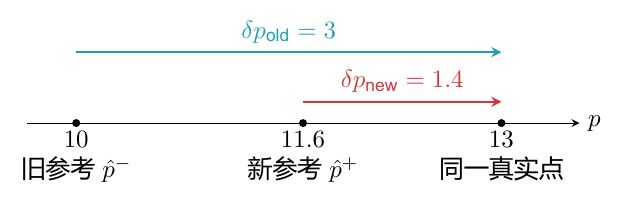
\includegraphics[width=.72\textwidth]{assets/images/附件-tikz-7-1.png}
\end{center}

\end{bookexample}

\begin{quote}

真实点没有因计算而移动。图中移动的是描述误差的零点，这就是注入与重置的区别。

\end{quote}

\subsection{从概率上看同一个循环}

第\ref{chap:md-07}章把分布看成给区域分配概率。预测让原来的可能状态随运动前进，并被过程噪声进一步分散；新观测到来后，能解释观测的候选状态获得更大的相对权重。例如两种候选位置原先各占一半，观测似然分别为$0.8$和$0.2$，归一化后权重就变为$0.8$和$0.2$。真实机器人没有被这次计算移动，改变的是我们的相信程度。

ESKF用局部线性化和高斯近似实现这个过程：$r,H$建立观测与误差的联系，$K$给出误差均值的修正，$P_u$给出后验的宽度，注入与重置再换回适合下一轮的表示。整个循环为

\begin{equation*}
(\hat x_k^+,P_k^+)
 \xrightarrow{\text{IMU预测}}(\hat x_{k+1}^-,P_{k+1}^-)
 \xrightarrow{\text{观测}}(d,P_u)
 \xrightarrow{\text{注入、重置}}(\hat x_{k+1}^+,P_{k+1}^+).
\end{equation*}

概率还可以帮助判断观测是否相容。若$m$维创新近似为$\mathcal N(0,S)$，将它按$S$白化后，各独立分量近似为标准正态；它们的平方和$r^\top S^{-1}r$就近似服从$\chi_m^2$。于是可以给"创新落在某椭球内"这个事件选择接收概率。这接上第\ref{chap:md-07}章的区域事件，具体门限推导留在下一章，不影响上述完整循环。

\section{回到同一台机器人：一次完整循环}

\subsection{每份数据在什么时候产生}

从$(\hat x_k^+,P_k^+)$出发，每个IMU样本先去偏置，推动名义状态；同一步的局部误差模型给出$\Phi_k,Q_{d,k}$，推动协方差。外部观测到来时，先计算预测观测$\hat z$、创新$r$及$H$，再由$S,K$得到误差修正$d$和观测后的协方差$P_u$。把$d$注入名义状态以后，使用$G_{\mathrm{reset}}$把协方差搬到新参考状态附近。保存的结果仍是一个合法状态和它附近的局部不确定性：

\begin{equation*}
(\hat x_k^+,P_k^+)
\xrightarrow{\text{IMU预测}}
(\hat x_{k+1}^-,P_{k+1}^-)
\xrightarrow{\text{观测、注入与重置}}
(\hat x_{k+1}^+,P_{k+1}^+).
\end{equation*}

\subsection{这个循环没有保存什么}

ESKF随着新数据到来，主要维护当前状态。它可以用先前的信息预测下一时刻，也可以在观测到来时修正当前估计；但这里没有把所有历史关键帧作为同一组未知量反复优化。若要把一段IMU读数留给后端多次评价，就需要第\ref{chap:md-10}章的预积分；若要让已经走远的轨迹因回到旧地点而整体调整，还需要第\ref{chap:md-12}章的后端与回环。
